\documentclass[10pt]{beamer}
% \documentclass[handout]{beamer}

\usetheme[progressbar=frametitle]{metropolis}
\usepackage{appendixnumberbeamer}
\setbeamercolor{background canvas}{bg=white}

\usepackage{booktabs}
\usepackage[scale=2]{ccicons}

\usepackage{pgfplots}
\usepackage{svg}
\usepgfplotslibrary{dateplot}

\usepackage{xspace}
\newcommand{\themename}{\textbf{\textsc{metropolis}}\xspace}

\usepackage{caption}
\usepackage{subcaption}

% -------symbols--------
\definecolor{cr}{RGB}{230, 92, 0}
\definecolor{red}{RGB}{255, 0, 0}
\newcommand{\ca}[1]{\textcolor{cr}{#1}}
\newcommand{\re}[1]{\textcolor{red}{#1}}

\usepackage{amsfonts, amsmath, amssymb, mathtools, latexsym, bbm}

% Teoremas, definições, proposições, lemas, corolários e conjecturas
% Pode dar conflito com outros pacotes
\usepackage{amsthm}

% conjuntos e indices
\newcommand{\blockset}{\mathcal{B}}
\newcommand{\blockcset}{\mathcal{B}_{c}}
\newcommand{\blockmset}{\mathcal{B'}}
\newcommand{\blockidx}{b}
\newcommand{\blocki}{b_i}
\newcommand{\blockj}{b_j}

\newcommand{\roomsete}{\mathcal{T}_{e}}
\newcommand{\roomseta}{\mathcal{T}_{a}}
\newcommand{\roomset}{\mathcal{T}}
\newcommand{\roomidx}{t}
\newcommand{\roomidxalt}{\ell}

\newcommand{\specialtyset}{\mathcal{S}}
\newcommand{\specialtytxset}{\mathcal{S}_{tx}}
\newcommand{\specialtyprset}{\mathcal{S}_{pr}}
\newcommand{\specialtycset}{\mathcal{S}_{ci}}
\newcommand{\specialtymset}{\mathcal{S}_{do}}
\newcommand{\specialtyidx}{s}

\newcommand{\planninghorizonset}{\mathcal{D}}
\newcommand{\planninghorizonidx}{d}

\newcommand{\timeperiodset}{\mathcal{N}}
\newcommand{\timeperiodidx}{n}

% --------------------------------------------------

% variaveis
\newcommand{\blockvar}{x_{\roomidx\blockidx\specialtyidx}}
\newcommand{\blockivar}{x_{\roomidx\blocki\specialtyidx}}
\newcommand{\blockjvar}{x_{\roomidx\blockj\specialtyidx}}
\newcommand{\deficitvar}{z_{\specialtyidx}}
\newcommand{\precvar}{y_{\roomidx\planninghorizonidx\specialtyidx}}
\newcommand{\integervar}{w_{\blockidx\specialtyidx}}
\newcommand{\balancevar}{L}

% --------------------------------------------------

% It doesn't need to be used, for now
% \newcommand{\surgeonset}{\mathcal{C}}
% \newcommand{\surgeonidx}{\ell}
% \newcommand{\anestset}{\mathcal{A}}
% \newcommand{\anestidx}{a}

% \newcommand{\surgeonvar}{y_{\surgeonidx\blockidx\roomidx}}
% \newcommand{\anestvar}{z_{\anestidx\blockidx\roomidx}}

% \newcommand{\surgeontospecialty}{\gamma}

% --------------------------------------------------

% parametros
\newcommand{\roomtospecialty}{\psi}
\newcommand{\demand}{\beta}
\newcommand{\numbersurgeons}{N}
\newcommand{\numbersanests}{\Gamma}
\newcommand{\needanest}{\gamma}
\newcommand{\revenue}{P}
\newcommand{\specteams}{\Phi}
\newcommand{\mindeficit}{\zeta}
\newcommand{\ub}{k}
\newcommand{\days}{|\planninghorizonset|}
\newcommand{\eps}{\epsilon}
\newcommand{\allowedrooms}{\alpha}
\newcommand{\entiredayroom}{\phi}


% ------------------------------------------------

\title{Programação Linear Inteira Aplicada ao Planejamento de Salas Cirúrgicas em Hospital Público}
\subtitle{João P. F. Silva, Lucas R. Bortoletto, Rafael C. S. Schouery, Edilson F. Arruda}
\date{13 de Março de 2025}
\titlegraphic{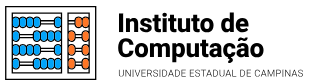
\includegraphics[height=0.9cm]{images/logo_ic.png}
    % \hfill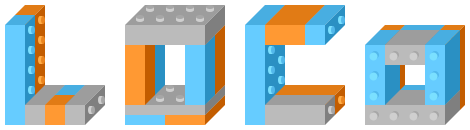
\includegraphics[height=0.8cm]{images/logo_loco.png}                
    \hfill
\includegraphics[height=1.2cm]{images/onpce.png}}

\begin{document}
\maketitle

\begin{frame}{HC Unicamp}
    \begin{columns}
        \column{0.5\textwidth}
        \begin{itemize}
            \setlength\itemsep{1em}
            \item<2-> Hospital que atende a população de Campinas e região
            \item<3-> Procedimentos de alta complexidade
            \item<4-> Mais de 30 especialidades cirúrgicas eletivas, incluindo de transplantes
            \item<5-> Hospital de ensino
        \end{itemize}
        \column{0.5\textwidth}
        \begin{figure}
            \centering
            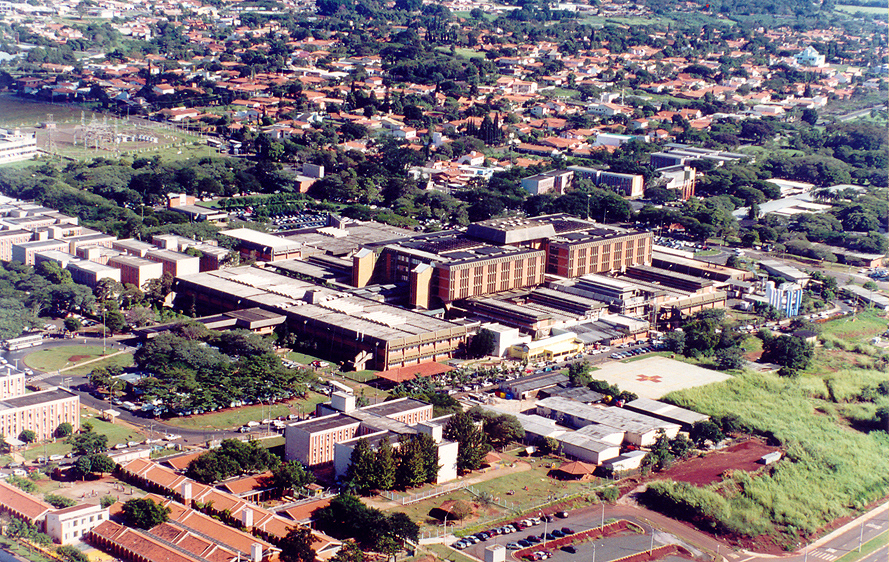
\includegraphics[width=0.8\textwidth]{images/aereahc.jpg}
            \caption{HC Unicamp}
        \end{figure}
    \end{columns}
\end{frame}


\begin{frame}{Gerenciamento do Centro Cirúrgico (CC)}
    \begin{columns}[t]
        \column{0.5\textwidth}
        \onslide<2->\textbf{Responsabilidades do CC}:
        \begin{itemize}
            \setlength\itemsep{1em}
            \item<3-> Alocação de equipes médicas
            \item<4-> Alocação de anestesistas (estatutário e PJ)
            \item<5-> Alocação de leitos
            \item<6-> Controle de estoque (leitos e fármacos)
            \item<7-> \ca{Planejamento de Salas Cirúrgicas}
        \end{itemize}
        \column{0.5\textwidth}
        \onslide<8->\textbf{Tarefas essenciais para:}
        \begin{itemize}
            \setlength\itemsep{1em}
            \item<9-> Otimização do uso dos recursos
            \item<10-> Redução de custos
            \item<11-> Aumento da eficiência
            \item<12-> Melhoria na qualidade do atendimento
        \end{itemize}
    \end{columns}
\end{frame}


\begin{frame}{Planejamento de Salas Cirúrgicas}
    \begin{columns}[t]
        \column{0.6\textwidth}
        \onslide<2->\textbf{O que é ``Planejar Salas Cirúrgicas''?}
        \begin{enumerate}
            \setlength\itemsep{.5em}
            \item[1-]<3-> Coletar disponibilidade de salas, anestesistas e equipes médicas
            \item[2-]<4-> Coletar demanda mínima das especialidades
            \item[3-]<5-> Alocar especialidades a blocos de tempo (manhã/tarde) a cada dia útil
            \item[4-]<6-> Em alguns casos, feito manualmente
        \end{enumerate}
        \column{0.4\textwidth}
        \onslide<5->\begin{figure}
            \centering
            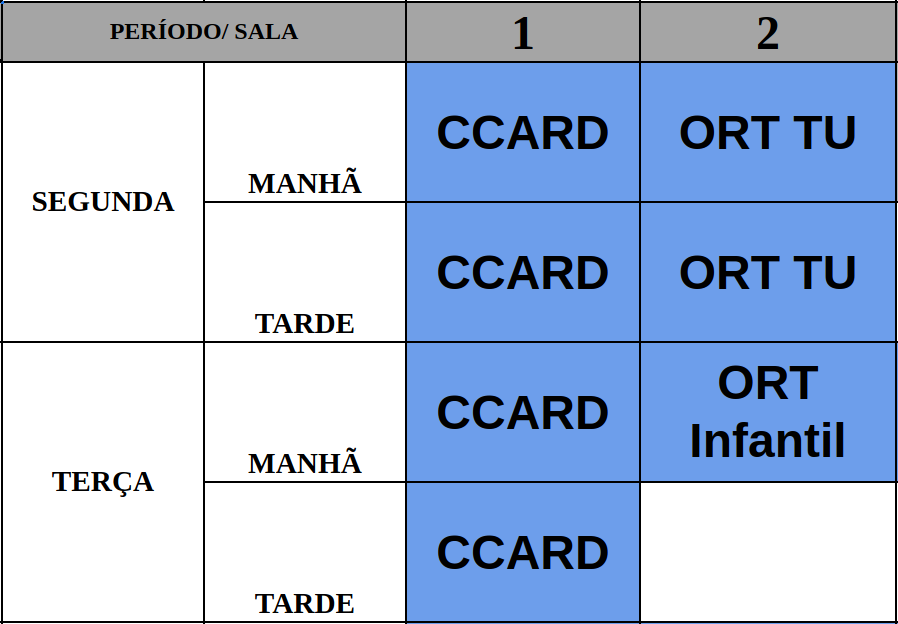
\includegraphics[width=0.8\textwidth]{images/schedule.png}
            \caption{Escala Cirúrgica\label{fig:schedule}}
        \end{figure}
    \end{columns}
\end{frame}


% \begin{frame}{Planejamento de Salas Cirúrgicas}
%     \begin{columns}[t]
%         \column{0.6\textwidth}
%         \onslide<2->\textbf{O que o planejamento afeta?}
%         \begin{itemize}
%             \setlength\itemsep{1em}
%             \item<3-> Redução do tempo de espera
%             \item<4-> Redução do tempo de ociosidade
%             \item<5-> Aumento da eficiência
%             \item<6-> ``Produção cirúrgica''
%         \end{itemize}
%         \column{0.4\textwidth}
%         \begin{figure}
%             \setcounter{figure}{\the\numexpr\value{figure}-1\relax}
%             \centering
%             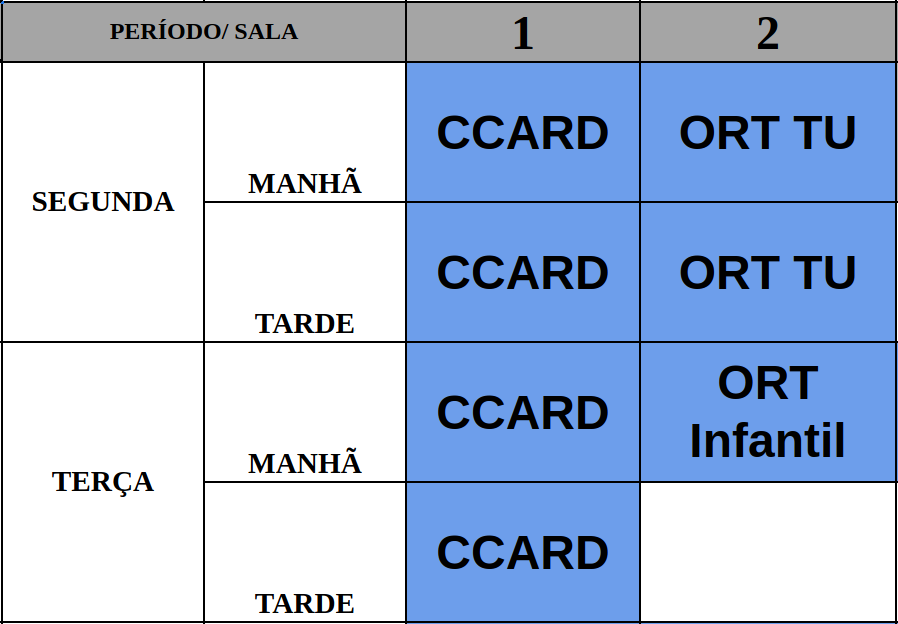
\includegraphics[width=0.8\textwidth]{images/schedule.png}
%             \caption{Escala Cirúrgica\label{fig:schedule}}
%             \setcounter{figure}{\the\numexpr\value{figure}+1\relax}
%         \end{figure}
%     \end{columns}
% \end{frame}


% \begin{frame}{Restrições de Planejamento}
%     Na literatura, as restrições envolvidas ao planejar a escala cirúrgica são muitas, a depender do hospital, período de planejamento, fluxo do paciente, entre outros. Algumas delas são:
%     \begin{itemize}
%         % \setlength\itemsep{1em}
%         \item Disponibilidade de salas
%         \item Disponibilidade de equipes médicas
%         \item Demanda mínima de cada especialidade
%         \item \alert{Disponibilidade de anestesistas}
%         \item \alert{Restrições de transplante}
%         \item Número de leitos (UTI/enfermaria) disponíveis
%         \item Disponibilidade de leitos
%         \item Tempo de recuperação
%         \item Tempo de limpeza
%         \item Tempo de preparação
%         \item Tempo de deslocamento
%     \end{itemize}
% \end{frame}

\begin{frame}{Modelo de Planejamento de Salas Cirúrgicas}
    \onslide<2->Considerando estas características e restrições, propomos um \ca{Modelo de Programação Linear Inteira Multiobjetivo para o Planejamento de Salas Cirúrgicas}
    \vspace{2em}

    \onslide<3->O caso de estudo do HC - Unicamp potencialmente traz o modelo para mais próximo da realidade
    \vspace{2em}

    \onslide<4->Temos a oportunidade de modelar diferentes funções objetivos (de acordo com as necessidades do hospital) mas a principal é a \ca{maximização da alocação de blocos}
\end{frame}

\begin{frame}{Variáveis do Modelo}
    \onslide<2->$\blockvar = \begin{cases}
        1\text{, caso a sala $\roomidx \in \roomset$, no bloco $\blockidx \in \blockset$, seja alocada para} \\
        \hspace{15em}\text{a especialidade $\specialtyidx \in \specialtyset$,} \\
        0\text{, caso contrário.}
    \end{cases}$
    \vspace{2em}

    \onslide<3->$\precvar = \begin{cases}
        1\text{, quando a sala $\roomidx$, no dia $\planninghorizonidx$, for alocada somente} \\
        \hspace{15em}\text{para a especialidade $\specialtyidx$,} \\
        0\text{, caso contrário.}
    \end{cases}$
\end{frame}


\begin{frame}{Variáveis do Modelo}
    \onslide<2->$\integervar := $ Número de transplantes a serem realizados dentro do período (garante paridade na quantidade de salas alocadas para transplante)
    \vspace{2em}

    \onslide<3->$\balancevar \in \mathbb{Z}$ := Variável utilizada para fazer balanceamento do número de alocações das especialidades. 
\end{frame}


\begin{frame}{Restrições do Modelo}
    \onslide<2->Cada especialidade precisa ser alocada a pelo menos $\mindeficit$ blocos (demanda mínima)
    \onslide<2->\begin{equation}
    \onslide<2->\label{eq:m2-2}
        \sum_{\roomidx \in \roomset} \sum_{\blockidx \in \blockset} \blockvar \geq \mindeficit{\specialtyidx} \hspace{2em} \forall\, \specialtyidx \in \specialtyset
    \end{equation}
    \vspace{2em}

    \onslide<3->Para cada especialidade $\specialtyidx \in \specialtyset$, a quantidade de blocos alocados no período de planejamento pode ser, no máximo, $k$ vezes maior do que a demanda $\demand_{\specialtyidx}$, com $k \in [0,1]$
    \onslide<3->\begin{equation}
    \label{eq:m2-3}
        \sum_{\roomidx \in \roomset} \sum_{\blockidx \in \blockset} \blockvar \leq (1 + \ub) \cdot \demand_{\specialtyidx} \hspace{2em} \forall\, \specialtyidx \in \specialtyset
    \end{equation}
\end{frame}


\begin{frame}{Restrições do Modelo}
    \onslide<2->Cada bloco de cada sala deve ser alocado a, no máximo, uma especialidade
    \onslide<2->\begin{equation}
    \label{eq:m2-4}
        \sum_{\specialtyidx \in \specialtyset} \blockvar \leq 1 \hspace{2em} \forall\, \roomidx \in \roomset,\, \blockidx \in \blockset
    \end{equation}
    \vspace{2em}

    \onslide<3->O número de alocações que precisam de anestesista ($\needanest_s = 1$) deve ser menor ou igual à quantidade de anestesistas disponíveis no bloco ($\numbersanests_{\blockidx}$)
    \onslide<3->\begin{equation}
    \label{eq:m2-5}
        \sum_{\roomidx \in \roomset} \sum_{\specialtyidx \in \specialtyset} \needanest_{\specialtyidx} \cdot \blockvar \leq \numbersanests_{\blockidx} \hspace{2em} \forall\, \blockidx \in \blockset
    \end{equation}
\end{frame}


\begin{frame}{Restrições do Modelo}
    \onslide<2->Cada especialidade só pode ser alocada em, no máximo, $\specteams$ salas, que é a quantidade de equipes disponíveis para aquela especialidade em um bloco
    \onslide<2->\begin{equation}
    \label{eq:m2-6}
        \sum_{\roomidx \in \roomset} \blockvar \leq \specteams_{\blockidx\specialtyidx} \hspace{2em} \forall\, \blockidx \in \blockset,\, \specialtyidx \in \specialtyset
    \end{equation}
    \vspace{2em}

    \onslide<3->Temos alguns casos de ter equipe disponível naquele bloco de horário, mas não em todas as salas, então temos o parâmetro $\allowedrooms_{\roomidx\blockidx\specialtyidx}$ para tratar esses casos
    \onslide<3->\begin{equation}
    \label{eq:m2-7}
        \blockvar = 0 \hspace{2em} \forall\, \roomidx \in \roomset,\,\blockidx \in \blockset,\, \specialtyidx \in \specialtyset : \allowedrooms_{\roomidx\blockidx\specialtyidx} = 0
    \end{equation}
\end{frame}
   

\begin{frame}{Restrições do Modelo}
    \onslide<2->Restrições para acoplar as variáveis de alocação $\blockvar$ e as variáveis de blocos sequenciais do mesmo dia $\precvar$
    % quando $\precvar = 0$, no máximo uma das variáveis de alocação do lado esquerdo será~$1$
    \onslide<2->\begin{align}
    \label{eq:m2-8}
        &\blockvar + x_{\roomidx(\blockidx+1)\specialtyidx} - 1 \leq \precvar \hspace{2em} \forall\, \roomidx \in \roomset,\, \blockidx \in \blockset,&\\
        & \hspace{4em}\,\specialtyidx \in \specialtyset,\, \planninghorizonidx \in \planninghorizonset : \text{ $\blockidx$ e $\blockidx+1$ são blocos do mesmo dia $\planninghorizonidx$}&\nonumber
    \end{align}

    % Acopla as variáveis de alocação $\blockvar$ e as variáveis de blocos sequenciais do mesmo dia $\precvar$, garantindo que quando $\precvar = 1$, as duas variáveis de alocação serão $1$
    \onslide<2->\begin{align}
    \label{eq:m2-9}
        &\blockvar + x_{\roomidx(\blockidx+1)\specialtyidx} \geq 2 \cdot \precvar \hspace{2em} \forall\, \roomidx \in \roomset,\, \blockidx \in \blockset,&\\
        &\hspace{4em}\,\specialtyidx \in \specialtyset,\, \planninghorizonidx \in \planninghorizonset : \text{ $\blockidx$ e $\blockidx+1$ são blocos do mesmo dia $\planninghorizonidx$}&\nonumber
    \end{align}
\end{frame}


\begin{frame}{Restrições do Modelo}
    \onslide<2->Especialidades que precisam de dois blocos (o dia todo) em alguns dias da semana
    \onslide<2->\begin{align}
    \label{eq:m2-10}
        &\blockvar = x_{\roomidx(\blockidx+1)\specialtyidx} \hspace{2em} \forall\, \roomidx \in \roomset,\, \blockidx \in \blockmset,&\\
        &\hspace{4em}\,\specialtyidx \in \specialtymset,\, \planninghorizonidx \in \planninghorizonset : \text{ $\blockidx$ e $\blockidx+1$ são blocos do mesmo dia $\planninghorizonidx$}&\nonumber
    \end{align}
    \vspace{2em}

    \onslide<3->Especialidades de transplante ($\specialtytxset$) precisam de duas salas alocadas no mesmo bloco de horário
    \onslide<3->\begin{equation}
    \label{eq:m2-11}
        \sum_{\roomidx \in \roomset} \blockvar = 2 \cdot \integervar \hspace{2em} \forall\, \blockidx \in \blockset,\, \specialtyidx \in \specialtytxset
    \end{equation}
\end{frame}


\begin{frame}{Restrições do Modelo}
    \onslide<2->Restrição que garante que as especialidades circunstanciais -- porém prioritárias -- precisam de blocos alocados em determinado intervalo de blocos $\blockcset$ (agendamento prévio)
    % (i.e., TMO que precisa de um bloco quando tem agendamento prévio)
    \onslide<2->\begin{equation}
    \label{eq:m2-12}
        \sum_{\roomidx \in \roomset} \sum_{\blockidx \in \blockcset} \blockvar = \demand_{\specialtyidx} \hspace{2em} \forall\, \specialtyidx \in \specialtycset
    \end{equation}
    \vspace{2em}

    \onslide<3->Restrição que faz com que todas as proporções de alocação sejam maiores do que uma variável $\balancevar$ (balanceamento)
    % Junto da segunda função objetivo, estaremos maximizando a menor proporção de alocação
    \onslide<3->\begin{equation}
    \label{eq:m2-13}
         \sum_{\roomidx \in \roomset} \sum_{\blockidx \in \blockset} \frac{\blockvar}{\demand_{\specialtyidx}} \geq \balancevar \hspace{2em} \forall\, \specialtyidx \in \specialtyset
    \end{equation}
\end{frame}


\begin{frame}{Funções Objetivo - Modelo Hierárquico}
    \begin{enumerate}
        \setlength\itemsep{2em}
        \onslide<2->\item Maximizar o número de alocações ($\blockvar$) de especialidades prioritárias $\specialtyprset$\\
        \vspace{0.5em}
        \onslide<2->Max $\displaystyle F_0 = \sum_{\roomidx \in \roomset} \sum_{\blockidx \in \blockset} \sum_{\specialtyidx \in \specialtyprset} \blockvar$ 

        \onslide<3->\item Maximizar o número de alocações ($\blockvar$), ou, em termos hospitalares, ``aumentar a produção cirúrgica''\\
        \vspace{0.5em}
        \onslide<3->Max $\displaystyle F_1 = \sum_{\roomidx \in \roomset} \sum_{\blockidx \in \blockset} \sum_{\specialtyidx \in \specialtyset} \blockvar$ 
    \end{enumerate}
\end{frame}

\begin{frame}{Funções Objetivo - Modelo Hierárquico}
    \begin{enumerate}
        \setlength\itemsep{2em}
        \onslide<2->\item[3.] Maximizar a menor proporção alocação/demanda, i.e., maximizar o menor valor de alocação proporcionalmente. Essa proporção é definida pela restrição~\ref{eq:m2-13}.\\
        \vspace{0.5em}  
        \onslide<2->Max $\displaystyle F_2 = \balancevar$

        \onslide<3->\item[4.] Maximizar a quantidade de especialidades alocadas sequencialmente no mesmo dia $\planninghorizonidx$ em uma sala $\roomidx$.\\
        \vspace{0.5em}
        \onslide<3->Max $\displaystyle F_3 = \sum_{\roomidx \in \roomset} \sum_{\planninghorizonidx \in \planninghorizonset} \sum_{\specialtyidx \in \specialtyset} \precvar$
    \end{enumerate}
\end{frame}


\begin{frame}{Resultados - Alocação de blocos}
    \begin{figure}
        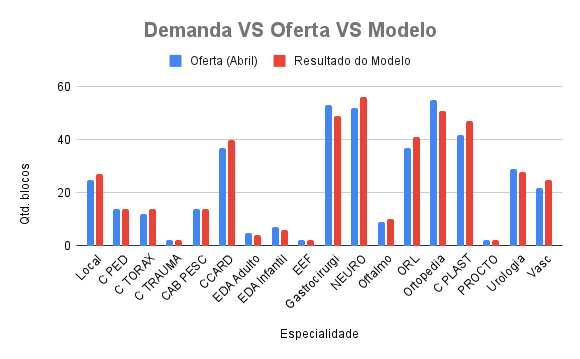
\includegraphics[width=0.8\textwidth]{images/esps_modelo.png}
    \end{figure}
\end{frame}


\begin{frame}{Resultados - Alocação de blocos}
    \begin{figure}
        \centering
        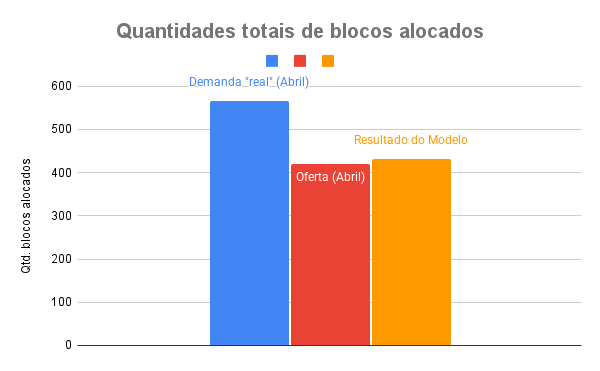
\includegraphics[width=0.8\textwidth]{images/totais_modelo.png}
    \end{figure}
    \onslide<2->Citavam que o principal gargalo era a falta de anestesistas, então exploramos esse parâmetro...
\end{frame}


\begin{frame}{Resultados - Mais Anestesistas}
    \begin{figure}
        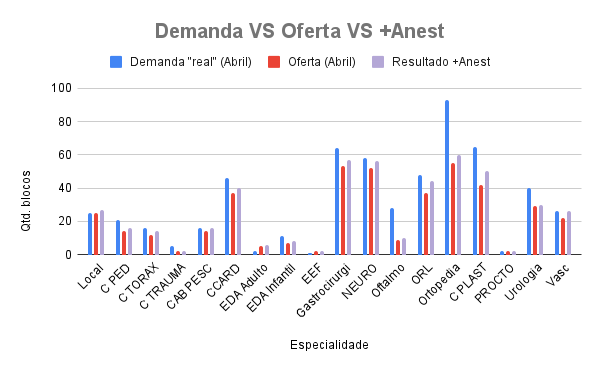
\includegraphics[width=0.8\textwidth]{images/esps_anest.png}
    \end{figure}
\end{frame}


\begin{frame}{Resultados - Mais Anestesistas}
    \begin{figure}
        \centering
        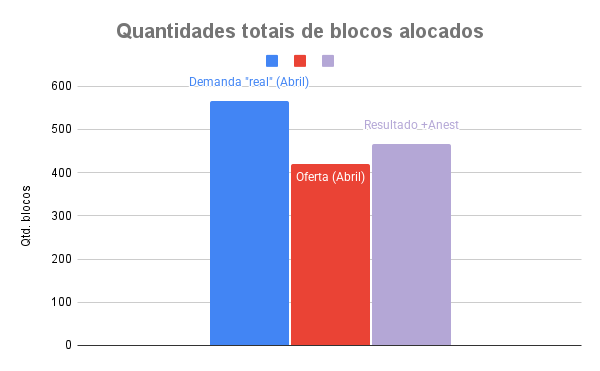
\includegraphics[width=0.8\textwidth]{images/totais_anest.png}
    \end{figure}
    \onslide<2->A quantidade de anestesistas é um gargalo, mas não o único...
\end{frame}


\begin{frame}{Conclusões}
    \begin{itemize}
        \setlength\itemsep{1em}
        \item<2-> Desenvolvemos um Modelo de Programação Linear Inteira Multiobjetivo para o Planejamento de Salas Cirúrgicas
        \item<3-> Modelo em fase de implantação no HC - Unicamp
        \begin{itemize}
            \item<4-> Open-source solver
        \end{itemize}
        \item<5-> \textbf{Dificuldades:} Dados reais do hospital são essenciais para a modelagem, porém exigem um grande esforço de coleta e tratamento
        \item<6-> \textbf{Trabalhos futuros:} Integrar o modelo com mais restrições reais (demanda/fila, tempos, leitos, ...) e explorar mais técnicas de otimização
    \end{itemize}
\end{frame}

\begin{frame}{Agradecimentos}
    \begin{columns}[t]
        \column{0.5\textwidth}
        \begin{figure}
            \centering
            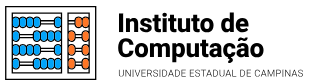
\includegraphics[width=0.8\textwidth]{images/logo_ic.png}
        \end{figure}
        \vspace{3em}
        \begin{figure}
            \centering
            
\includegraphics[width=0.8\textwidth]{images/fapesp.png}
        \end{figure}
        \column{0.5\textwidth}
        \begin{figure}
            \centering
            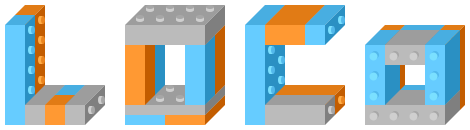
\includegraphics[width=0.8\textwidth]{images/logo_loco.png}
        \end{figure}
        \begin{figure}
            \centering
            
\includegraphics[width=0.7\textwidth]{images/onpce.png}
        \end{figure}
    \end{columns}
\end{frame}

\end{document}
